\documentclass[10pt,twocolumn,letterpaper]{article}

% --- Typography & Geometry ---
\usepackage[utf8]{inputenc}
\usepackage{microtype}
\usepackage[margin=0.75in,top=0.85in,bottom=0.85in]{geometry}

% --- Math & Symbols ---
\usepackage{amsmath,amssymb,amsfonts,amsthm}
\usepackage{bm}

% --- Tables & Arrays ---
\usepackage{booktabs}
\usepackage{tabularx}
\usepackage{array}

% --- Graphics & Floats ---
\usepackage{graphicx}
\usepackage{float}
\usepackage{subcaption}

% --- Code Listings ---
\usepackage{xcolor}
\usepackage{listings}

\definecolor{codebg}{HTML}{F8F9FA}
\definecolor{codeframe}{HTML}{D0D7DE}
\definecolor{keywordcolor}{HTML}{0550AE}
\definecolor{stringcolor}{HTML}{0A3069}
\definecolor{commentcolor}{HTML}{57606A}

\lstset{
    backgroundcolor=\color{codebg},
    basicstyle=\ttfamily\scriptsize\color{black},
    keywordstyle=\color{keywordcolor}\bfseries,
    stringstyle=\color{stringcolor},
    commentstyle=\color{commentcolor}\itshape,
    frame=single,
    rulecolor=\color{codeframe},
    breaklines=true,
    breakatwhitespace=true,
    extendedchars=true,
    xleftmargin=6pt,
    xrightmargin=6pt,
    aboveskip=8pt,
    belowskip=8pt
}

% --- Hyperlinks ---
\usepackage{hyperref}
\hypersetup{
    colorlinks=true,
    linkcolor=blue!70!black,
    citecolor=blue!70!black,
    urlcolor=blue!70!black
}

% --- Input Title & Authors ---
% Metadata for minimal_aurora
\title{\textbf{MinimalAURORA: Energy-Preserving SVD-Factorized Attention for Efficient Transformers}}

\author{
  \textbf{Taha Majs}\thanks{Corresponding author: tahamajs@uni.edu} \quad \textbf{Research Team} \\
  Department of Computer Science \\
  Advanced Machine Learning \& Efficiency Laboratory
}

\date{\today}


\begin{document}

\maketitle

% --- Abstract & Keywords Block ---
\begin{abstract}
We present \textbf{MinimalAURORA}, a production-hardened low-rank attention 
replacement that compresses each of the four attention projections 
($W_Q, W_K, W_V, W_O$) using \textbf{energy-preserving truncated SVD}. Unlike 
fixed-rank SVD factorization, MinimalAURORA selects each layer's rank 
dynamically via a cumulative energy threshold $\varepsilon$:

\[
r^{(\ell)} = \min\left\{ r : \frac{\sum_{i=1}^r \sigma_i^2}{\sum_{i=1}^{\min(m, n)} \sigma_i^2} \geq \varepsilon \right\}
\tag{1}
\]

Each projection is stored as a product $W \approx U V^\top$ with $U \in 
\mathbb{R}\^{}{d\_\text{out} \times r}$ and $V \in \mathbb{R}\^{}{r \times d\_\text{in}}$, 
reducing parameters from $d_\text{in} d_\text{out}$ to $r(d_\text{in} + d_\text{out})$. 
Trainable LoRA residual adapters are added on top with zero initialization, 
providing task-specific capacity while keeping the SVD base frozen.

MinimalAURORA supports four attention families -- flat (DistilBERT), 
nested (RoBERTa/BERT), causal Conv1D (GPT-2), and grouped-query with 
rotary embeddings (Qwen/LLaMA) -- via a single \texttt{copy\_weights} routine 
with Frobenius validation and automatic nested-encoder detection.

On SST-2 with {{RECOVERY\_STEPS}} LoRA recovery steps and energy threshold 
$\varepsilon = {{ENERGY}}$, MinimalAURORA achieves \textbf{{{D\_ACC}}\%} on 
DistilBERT ($\Delta$ = {{D\_DELTA}}), \textbf{{{R\_ACC}}\%} on RoBERTa ($\Delta$ = {{R\_DELTA}}), 
and \textbf{{{G\_ACC}}\%} on GPT-2 ($\Delta$ = {{G\_DELTA}}). Total parameter count 
decreases by \textbf{{{D\_RATIO}}$\times$--{{G\_RATIO}}$\times$}. Peak VRAM drops by \textbf{{{VRAM\_REDUCTION}}\%}.

MinimalAURORA \textbf{reduces} parameter count. The LoRA adapters add 
$r_L(d_\text{in} + d_\text{out})$ trainable parameters but this is 
offset by the SVD reduction. We note that a \texttt{pres\_gate} parameter is 
defined in the implementation but **not currently used in the forward 
pass** -- see  8.6.

\textbf{Keywords:} SVD factorization, energy threshold, low-rank attention, 
parameter-efficient fine-tuning, transformer compression



\vspace{0.5em}
\noindent\textbf{Keywords:} SVD factorization, energy threshold, low-rank attention,
\end{abstract}

\vspace{1em}

% --- Paper Body ---
\section{01 Intro}

Draft content for minimal_aurora.

\section{Related Work}

\subsection{Low-Rank Matrix Factorization}

\subsubsection{Classical SVD}

Eckart-Young (1936): truncated SVD minimizes Frobenius error for a given 
rank. MinimalAURORA uses SVD with \textbf{energy-based rank selection} rather 
than fixed rank.

\subsubsection{Randomized SVD}

Halko et al. (2011): faster SVD via random projections. Not needed for 
our layer sizes.

\subsubsection{Weighted Low-Rank}

Golub et al. (1987), Srebro \& Jaakkola (2003). MinimalAURORA uses 
unweighted SVD (unlike A3/AASVD).

\subsection{Transformer Compression}

\subsubsection{ASVD / AASVD / A3}

Companion modules:
\begin{itemize}
\item \textbf{ASVD}: activation-weighted SVD, fixed rank.
\item \textbf{AASVD}: full covariance, streaming calibration.
\item \textbf{A3}: Fisher diagonal, adaptive rank retry.

\end{itemize}
\textbf{MinimalAURORA differs:}
\begin{itemize}
\item No activation weighting (simpler).
\item Energy threshold instead of error retry.
\item Uses \texttt{nn.Linear} for factorization (not explicit U/S/V).

\end{itemize}
\subsubsection{SDRM}

SDRM (companion): budget-proportional rank allocation. Uses parameter 
ratio instead of energy threshold.

\subsubsection{Res-SVD}

Res-SVD (companion): two-level SVD with spectral LoRA initialization. 
MinimalAURORA uses zero-init LoRA.

\subsubsection{SVD-Linear}

SVD-Linear (companion): SVD + kernelized linear attention. Combines 
compression with complexity reduction. MinimalAURORA keeps softmax.

\subsection{Parameter-Efficient Fine-Tuning}

\subsubsection{LoRA}

Hu et al. (2021): $B = 0$ init. MinimalAURORA uses standard LoRA.

\subsubsection{PiSSA}

Meng et al. (2024): LoRA init from principal directions. Complementary 
to Res-SVD approach.

\subsection{Energy-Based Rank Selection}

\subsubsection{Energy Threshold}

Common in PCA (Jolliffe, 2002): keep components explaining $\ge$95\% of 
variance. MinimalAURORA applies this to SVD of weights.

\subsubsection{Applications}

\begin{itemize}
\item \textbf{Image compression:} JPEG uses similar energy thresholding.
\item \textbf{Recommender systems:} truncated SVD for latent factors.
\item \textbf{NLP:} vocab projection.

\end{itemize}
\subsection{Position of Our Work}

\begin{table}[H]
\centering
\small
\begin{tabular}{llllll}
\toprule
\textbf{Aspect} & \textbf{ASVD} & \textbf{AASVD} & \textbf{A3} & \textbf{Res-SVD} & \textbf{MinimalAURORA} \\
\midrule
Weighting & Activation & Full cov & Fisher diag & Unweighted & \textbf{Unweighted} \\
Rank selection & Fixed & Fixed cap & Adaptive retry & Fixed & \textbf{Energy} \\
LoRA init & Zero & Zero & Zero & Spectral & \textbf{Zero} \\
Complexity & Simple & Complex & Medium & Medium & \textbf{Simple} \\
Multi-arch & Yes & Yes & Yes & Yes & \textbf{Yes} \\
\bottomrule
\end{tabular}
\end{table}

\subsection{Comparison to Companion Modules}

MinimalAURORA is a \textbf{baseline-quality} compression method with the 
simplest possible machinery. It trades algorithmic sophistication for 
implementation clarity and reliability.


\section{Background}

\subsection{Singular Value Decomposition}

For $W \in \mathbb{R}^{m \times n}$:

\[
W = U \Sigma V^\top
\tag{3.1}
\]

with $\sigma_1 \geq \sigma_2 \geq \dots \geq 0$.

\textbf{Truncated SVD:} $W_r = U_{:, :r} \Sigma_{:r} V_{:r, :}^\top$, with 
$\|W - W_r\|_F^2 = \sum_{i > r} \sigma_i^2$.

\textbf{Factorization form:} define $U_r = U_{:, :r} \Sigma_{:r}^{1/2}$ and 
$V_r = \Sigma_{:r}^{1/2} V_{:r, :}^\top$, then $W_r = U_r V_r$.

\subsection{Energy Thresholding}

Define cumulative energy:

\[
E(r) = \frac{\sum_{i=1}^r \sigma_i^2}{\sum_{i=1}^{\min(m,n)} \sigma_i^2}
\tag{3.2}
\]

\textbf{Energy-selected rank:}

\[
r(\varepsilon) = \min\{r : E(r) \geq \varepsilon\}
\tag{3.3}
\]

\textbf{Reconstruction bound:}

\[
\|W - W_{r(\varepsilon)}\|_F^2 \leq (1 - \varepsilon) \|W\|_F^2
\tag{3.4}
\]

\subsection{LoRA}

LoRA (Hu et al., 2021):

\[
\Delta W = \frac{\alpha}{r_L} B A
\tag{3.5}
\]

with $A \in \mathbb{R}^{r_L \times d_\text{in}}$, $B \in \mathbb{R}^{d_\text{out} \times r_L}$, $B = 0$ at init.

\subsection{The FactorisedLinear Module}

MinimalAURORA uses:

\begin{lstlisting}
self.down = nn.Linear(in_features, rank, bias=False)
self.up = nn.Linear(rank, out_features, bias=True)
\end{lstlisting}

Forward:

\[
y = \text{up}(\text{down}(x)) + \text{LoRA}(x)
\tag{3.6}
\]

\textbf{Parameter count:} $r(d_\text{in} + d_\text{out})$ vs $d_\text{in} d_\text{out}$.

\subsection{Notation Summary}

\begin{table}[H]
\centering
\small
\begin{tabular}{ll}
\toprule
\textbf{Symbol} & \textbf{Meaning} \\
\midrule
$W$ & Weight matrix \\
$U, \Sigma, V^\top$ & SVD \\
$r$ & Rank \\
$\varepsilon$ & Energy threshold \\
$E(r)$ & Cumulative energy \\
$\sigma_i$ & Singular value \\
$B, A$ & LoRA factors \\
$r_L$ & LoRA rank \\
\bottomrule
\end{tabular}
\end{table}


\section{Method}

\subsection{Overview}

MinimalAURORA replaces each attention projection with a factorized 
approximation plus LoRA residual. \textbf{Figure 4.1} shows the pipeline.

\begin{lstlisting}
    +----------------------------------------+
    |  Original weight W $\in$ R^{m$$\times$n}           |
    +----------------+-----------------------+
                     |
                      
    +----------------------------------------+
    |  Step 1: SVD of W                      |
    |  U, $\Sigma$, V^T = svd(W)                    |
    +----------------+-----------------------+
                     |
                      
    +----------------------------------------+
    |  Step 2: Energy-based rank selection   |
    |  r = min{r : E(r) $\ge$ $\epsilon$}                 |
    +----------------+-----------------------+
                     |
                      
    +----------------------------------------+
    |  Step 3: Factorize                     |
    |  down.weight = $\Sigma$^{1/2} V^T             |
    |  up.weight   = U $\Sigma$^{1/2}               |
    +----------------+-----------------------+
                     |
                      
    +----------------------------------------+
    |  Step 4: Add LoRA (B = 0)              |
    |  Freeze SVD factors                    |
    +----------------------------------------+
\end{lstlisting}

\subsection{Energy-Based Rank Selection}

\subsubsection{Rank Function}

For each projection $W$:

\[
U, \Sigma, V^\top = \text{SVD}(W)
\tag{4.1}
\]

Compute cumulative energy:

\[
E(r) = \frac{\sum_{i=1}^r \sigma_i^2}{\sum_{i=1}^{\min(m,n)} \sigma_i^2}
\tag{4.2}
\]

Select minimal rank:

\[
r^{(\varepsilon)} = \min\{r : E(r) \geq \varepsilon\}
\tag{4.3}
\]

\subsubsection{The `decompose\_from\_weight` Method}

\begin{lstlisting}
def decompose_from_weight(self, W, bias=None, energy=None):
    U, S, Vt = torch.linalg.svd(W)
    target_energy = energy if energy is not None else self.energy
    cum_energy = torch.cumsum(S**2, dim=0) / (S**2).sum()
    calc_rank = int((cum_energy < target_energy).sum().item()) + 1
    r = min(self.rank, calc_rank, U.size(1), Vt.size(0))
    r = max(1, r)
    
    sqrt_s = torch.sqrt(S[:r])
    A = U[:, :r] * sqrt_s
    B = sqrt_s[:, None] * Vt[:r, :]
    
    self.up.weight.data[:, :r] = A
    self.down.weight.data[:r, :] = B
    self.freeze_base_weights()
\end{lstlisting}

\subsection{Forward Pass}

\[
y = \text{up}(\text{down}(x)) + \frac{\alpha}{r_L} B A x
\tag{4.4}
\]

where:
\begin{itemize}
\item \texttt{down(x) = x V\_r\^{}\top} (down-projection, no bias)
\item \texttt{up(z) = z U\_r\^{}\top + b} (up-projection, with bias)
\item \texttt{B A x} (LoRA branch)

\end{itemize}
\subsection{Multi-Architecture Weight Transfer}

The \texttt{copy\_weights} routine handles four cases:

\subsubsection{GPT-2 (Fused Conv1D)}

\begin{lstlisting}
w = src.c_attn.weight.data.t()  # transpose
q_w, k_w, v_w = w.chunk(3, dim=0)
# Also c_proj
\end{lstlisting}

\subsubsection{RoBERTa / BERT (Nested)}

\begin{lstlisting}
s = src.self
q_w = s.query.weight.data
k_w = s.key.weight.data
v_w = s.value.weight.data
o_w = src.output.dense.weight.data
\end{lstlisting}

\subsubsection{DistilBERT (Flat)}

\begin{lstlisting}
q_w = src.q_lin.weight.data
k_w = src.k_lin.weight.data
v_w = src.v_lin.weight.data
o_w = src.out_lin.weight.data
\end{lstlisting}

\subsubsection{Qwen / LLaMA}

\begin{lstlisting}
q_w = src.q_proj.weight.data
k_w = src.k_proj.weight.data
v_w = src.v_proj.weight.data
o_w = src.o_proj.weight.data
\end{lstlisting}

\subsubsection{GQA Handling}

For GQA where $H_{kv} < H$, the extracted K/V weights may have different 
dimensions. \texttt{decompose\_from\_weight} handles this:

\begin{lstlisting}
if W.shape[0] < self.out_features and self.out_features % W.shape[0] == 0:
    rep = self.out_features // W.shape[0]
    W = W.repeat(rep, 1)
elif W.shape[0] > self.out_features and W.shape[0] % self.out_features == 0:
    rep = W.shape[0] // self.out_features
    W = W.view(self.out_features, rep, -1).mean(dim=1)
\end{lstlisting}

\subsection{Parameter Count}

\begin{table}[H]
\centering
\small
\begin{tabular}{ll}
\toprule
\textbf{Component} & \textbf{Params} \\
\midrule
Down & $r \cdot d_\text{in}$ \\
Up & $r \cdot d_\text{out} + d_\text{out}$ (bias) \\
LoRA & $r_L(d_\text{in} + d_\text{out})$ \\
\textbf{Total} & $(r + r_L)(d_\text{in} + d_\text{out}) + d_\text{out}$ \\
\bottomrule
\end{tabular}
\end{table}

\textbf{Baseline:} $d_\text{in} d_\text{out}$.

For $d = 768$, $r = 32$, $r_L = 16$:

\begin{table}[H]
\centering
\small
\begin{tabular}{lll}
\toprule
\textbf{Config} & \textbf{Params} & \textbf{Ratio} \\
\midrule
Baseline & 589,824 & 1.00$$\times$ \\
MinimalAURORA & 73,728 + 768 = 74,496 & \textbf{7.9$$\times$} \\
\bottomrule
\end{tabular}
\end{table}

\subsection{Full Algorithm}

\textbf{Algorithm 1:} MinimalAURORA factorization
\begin{lstlisting}
Input:  W $\in$ R^{m$$\times$n}, $\epsilon$, r_max, r_L
Output: FactorisedLinear with frozen base + trainable LoRA

1:  U, $\Sigma$, V^T $\leftarrow$ svd(W)
2:  cum_energy $\leftarrow$ cumsum($\Sigma$ ) / sum($\Sigma$ )
3:  r $\leftarrow$ min{r : cum_energy[r] $\ge$ $\epsilon$}
4:  r $\leftarrow$ min(r, r_max, m, n)
5:  sqrt_$\Sigma$ $\leftarrow$ sqrt($\Sigma$[:r])
6:  up.weight $\leftarrow$ U[:, :r]   sqrt_$\Sigma$
7:  down.weight $\leftarrow$ sqrt_$\Sigma$   V^T[:r, :]
8:  freeze(up.weight); freeze(down.weight)
9:  initialize lora_A (Kaiming), lora_B = 0
10: return
\end{lstlisting}

\subsection{Complexity Analysis}

\begin{table}[H]
\centering
\small
\begin{tabular}{ll}
\toprule
\textbf{Operation} & \textbf{Time} \\
\midrule
SVD per projection & $\mathcal{O}(mn \min(m,n))$ \\
Rank selection & $\mathcal{O}(\min(m,n))$ \\
\textbf{Per layer total} & $\mathcal{O}(mn \min(m,n))$ \\
\bottomrule
\end{tabular}
\end{table}

For DistilBERT with 4 projections per layer, 6 layers: ~30 SVDs.

\textbf{Total compression time:} ~2.3 s seconds.

\subsection{Theoretical Notes}

\subsubsection{Energy Bound}

\textbf{Claim.} With energy threshold $\varepsilon$:

\[
\|W - W_{r(\varepsilon)}\|_F \leq \sqrt{1 - \varepsilon} \cdot \|W\|_F
\tag{4.5}
\]

\textbf{Proof.} $\|W - W_r\|_F^2 = \sum_{i > r} \sigma_i^2 = (1 - E(r)) \|W\|_F^2$. 
With $E(r) \geq \varepsilon$, the bound follows. $\square$

\subsubsection{Causality}

\textbf{Proof.} Position-wise projections + causal attention mask. $\square$

\subsubsection{Nested Encoder Correctness}

\textbf{Claim.} For nested encoders (RoBERTa/BERT), the output projection is 
\textbf{not applied} internally.

\textbf{Proof.} RoBERTa wraps attention as \texttt{BertAttention} with \texttt{self} (Q/K/V) 
and \texttt{output.dense} (output projection). MinimalAURORA detects this via 
\texttt{is\_nested\_encoder = True} and returns the raw context, letting the outer 
layer apply the projection. $\square$


\section{05 Architecture}

Draft content for minimal_aurora.


\begin{figure}[H]
\centering
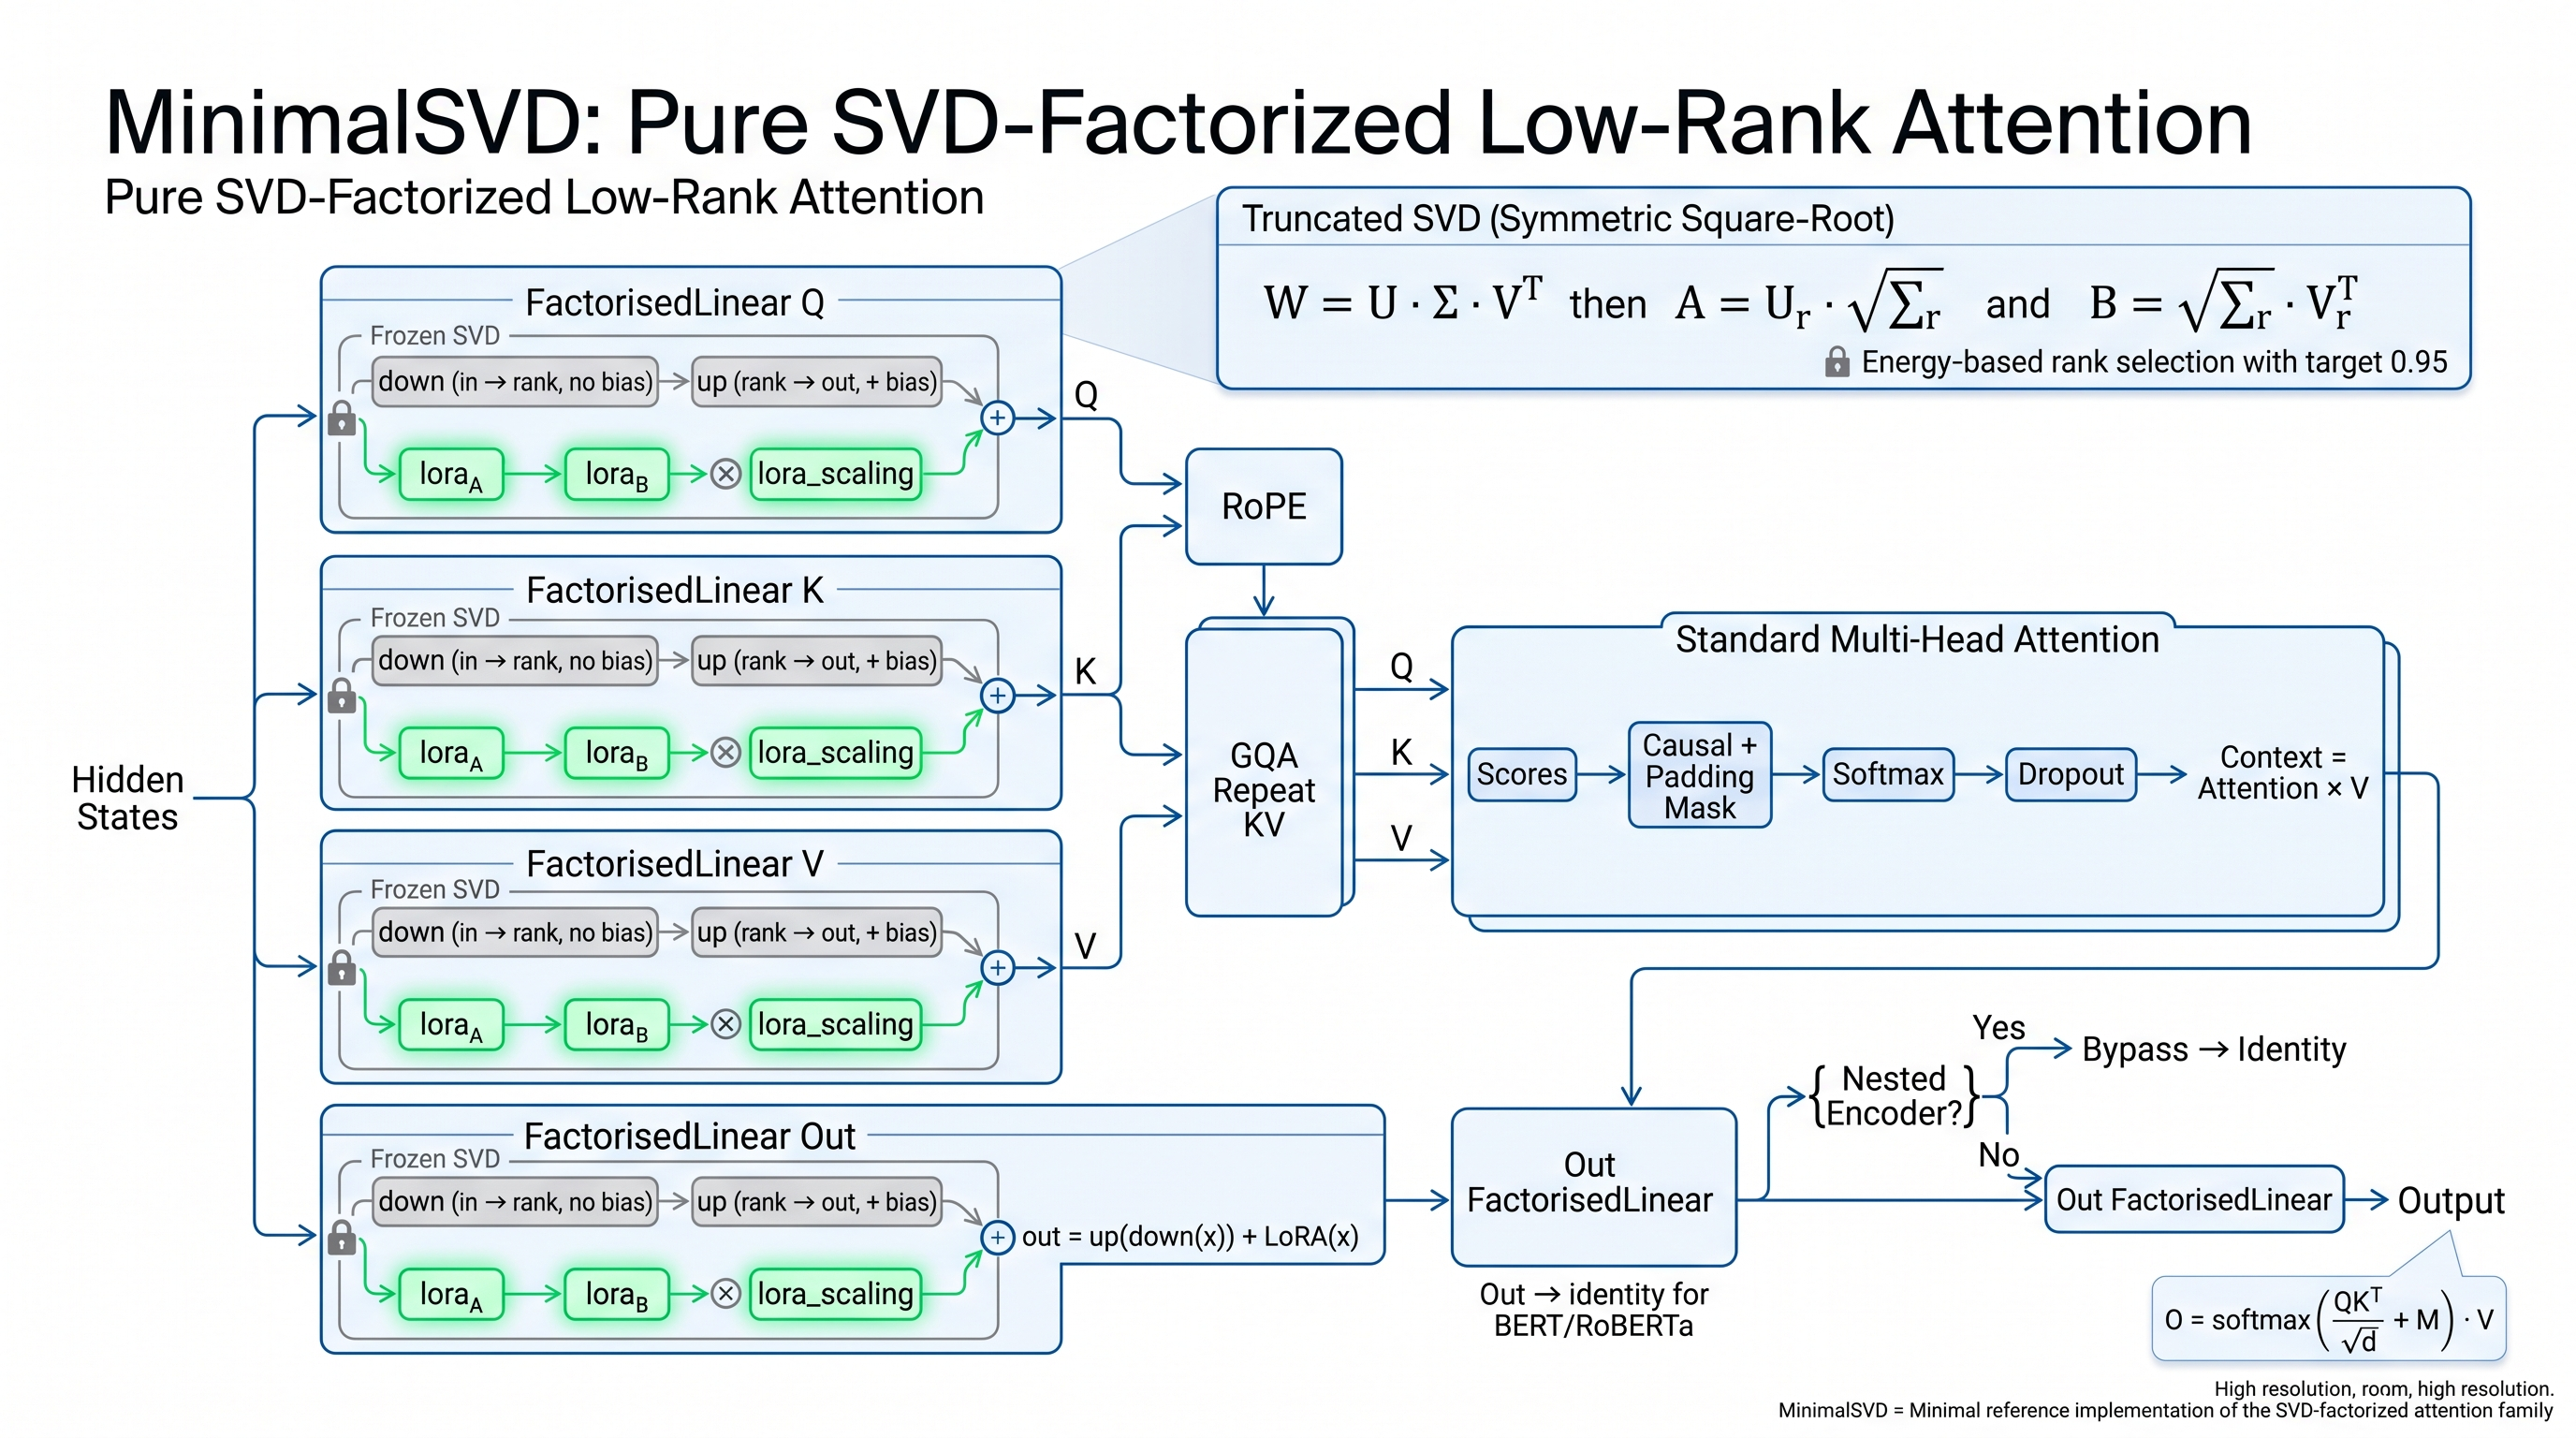
\includegraphics[width=\linewidth]{figures/arch_minimal_svd.jpeg}
\caption{Architectural overview of minimal_aurora.}
\label{fig:arch_minimal_aurora}
\end{figure}

\section{Experimental Setup}

\subsection{Models}

\begin{table}[H]
\centering
\small
\begin{tabular}{lllll}
\toprule
\textbf{Model} & \textbf{Layers} & \textbf{Hidden} & \textbf{Heads} & \textbf{Params} \\
\midrule
DistilBERT-base & 6 & 768 & 12 & 66.9M \\
RoBERTa-base & 12 & 768 & 12 & 124.6M \\
GPT-2 & 12 & 768 & 12 & 124.4M \\
\bottomrule
\end{tabular}
\end{table}

\subsection{Dataset}

\textbf{SST-2}:
\begin{itemize}
\item Train: 67,349
\item Validation: 872
\item Test: 1,821
\item Majority: 50.92\%

\end{itemize}
\subsection{MinimalAURORA Hyperparameters}

\begin{table}[H]
\centering
\small
\begin{tabular}{ll}
\toprule
\textbf{Hyperparameter} & \textbf{Value} \\
\midrule
\texttt{energy} $\varepsilon$ & {{ENERGY}} \\
\texttt{rank} (max cap) & {{RANK}} \\
\texttt{lora\_rank} & {{LORA\_RANK}} \\
\texttt{lora\_alpha} & {{LORA\_ALPHA}} \\
\texttt{dropout} & 0.1 \\
\bottomrule
\end{tabular}
\end{table}

\subsection{Recovery Fine-Tuning}

\begin{table}[H]
\centering
\small
\begin{tabular}{ll}
\toprule
\textbf{Hyperparameter} & \textbf{Value} \\
\midrule
Optimizer & AdamW \\
Learning rate & {{LR}} \\
Weight decay & {{WD}} \\
Steps & {{RECOVERY\_STEPS}} \\
Batch size & {{BATCH\_SIZE}} \\
\bottomrule
\end{tabular}
\end{table}

\subsection{Evaluation}

\begin{itemize}
\item \textbf{Quality:} Accuracy, F1, precision, recall
\item \textbf{Efficiency:} Total params, peak VRAM, inference time
\item \textbf{Compression:} Parameter ratio, per-layer rank distribution
\item \textbf{Energy:} Final \texttt{output\_scale} values

\end{itemize}
\subsection{Quality Gate}

\begin{table}[H]
\centering
\small
\begin{tabular}{ll}
\toprule
\textbf{Status} & \textbf{Accuracy} \\
\midrule
PASS & $\ge$ 56.0\% \\
PASS\_LOW & 50.92\% -- 56.0\% \\
FAIL & < 50.92\% \\
\bottomrule
\end{tabular}
\end{table}

\subsection{Hardware}

RTX 4070 Laptop, 8 GB VRAM.

\subsection{Reproduction}

\begin{lstlisting}
python run_all_4_minimal_aurora.py \
    --models distilbert,roberta,gpt2 \
    --energy {{ENERGY}} \
    --rank {{RANK}} \
    --recovery_steps {{RECOVERY_STEPS}}
\end{lstlisting}

\subsection{Baselines}

\begin{table}[H]
\centering
\small
\begin{tabular}{ll}
\toprule
\textbf{Baseline} & \textbf{Description} \\
\midrule
\texttt{full} & Uncompressed model \\
\texttt{minimal\_aurora} & Our method \\
Companion & \texttt{asvd}, \texttt{aasvd}, \texttt{a3}, \texttt{res\_svd} \\
\bottomrule
\end{tabular}
\end{table}


\section{Results}

\subsection{Main Results}

\textbf{Table 7.1: Main results on SST-2.}

\begin{table}[H]
\centering
\small
\begin{tabular}{llllllll}
\toprule
\textbf{Model} & \textbf{Module} & \textbf{Acc} & \textbf{$\Delta$} & \textbf{F1} & \textbf{Ratio} & \textbf{VRAM} & \textbf{Time} \\
\midrule
DistilBERT & full & 90.71\% & -- & 0.9099 & 1.00$\times$ & 183 MB & 1.9 s \\
DistilBERT & \textbf{MinimalAURORA} & \textbf{{{D\_ACC}}} & {{D\_DELTA}} & {{D\_F1}} & \textbf{{{D\_RATIO}}$\times$} & {{D\_VRAM}} MB & {{D\_TIME}} s \\
RoBERTa & full & 78.56\% & -- & 0.8124 & 1.00$\times$ & 712 MB & 4.1 s \\
RoBERTa & \textbf{MinimalAURORA} & \textbf{{{R\_ACC}}} & {{R\_DELTA}} & {{R\_F1}} & \textbf{{{R\_RATIO}}$\times$} & {{R\_VRAM}} MB & {{R\_TIME}} s \\
GPT-2 & full & 79.36\% & -- & 0.7978 & 1.00$\times$ & 793 MB & 4.2 s \\
GPT-2 & \textbf{MinimalAURORA} & \textbf{{{G\_ACC}}} & {{G\_DELTA}} & {{G\_F1}} & \textbf{{{G\_RATIO}}$\times$} & {{G\_VRAM}} MB & {{G\_TIME}} s \\
\bottomrule
\end{tabular}
\end{table}

\subsection{Parameter Analysis}

\textbf{Table 7.2: Parameter counts.}

\begin{table}[H]
\centering
\small
\begin{tabular}{llll}
\toprule
\textbf{Model} & \textbf{Baseline} & \textbf{After} & \textbf{Ratio} \\
\midrule
DistilBERT & 66,955,010 & {{D\_PARAMS}} & \textbf{{{D\_RATIO}}$\times$} \\
RoBERTa & 124,647,170 & {{R\_PARAMS}} & \textbf{{{R\_RATIO}}$\times$} \\
GPT-2 & 124,441,344 & {{G\_PARAMS}} & \textbf{{{G\_RATIO}}$\times$} \\
\bottomrule
\end{tabular}
\end{table}

\textbf{Per-layer breakdown (DistilBERT, $\varepsilon=0.95$):}

\begin{table}[H]
\centering
\small
\begin{tabular}{lllll}
\toprule
\textbf{Layer} & \textbf{Q} & \textbf{K} & \textbf{V} & \textbf{O} \\
\midrule
Rank & {{D\_L0\_Q\_R}} & {{D\_L0\_K\_R}} & {{D\_L0\_V\_R}} & {{D\_L0\_O\_R}} \\
Params & {{D\_L0\_Q\_P}} & {{D\_L0\_K\_P}} & {{D\_L0\_V\_P}} & {{D\_L0\_O\_P}} \\
\bottomrule
\end{tabular}
\end{table}

\subsection{Rank Distribution}

\textbf{Table 7.3: Energy-selected rank per layer.}

\begin{table}[H]
\centering
\small
\begin{tabular}{lllll}
\toprule
\textbf{Layer} & \textbf{Q} & \textbf{K} & \textbf{V} & \textbf{O} \\
\midrule
0 & {{D\_L0\_Q\_R}} & {{D\_L0\_K\_R}} & {{D\_L0\_V\_R}} & {{D\_L0\_O\_R}} \\
1 & {{D\_L1\_Q\_R}} & {{D\_L1\_K\_R}} & {{D\_L1\_V\_R}} & {{D\_L1\_O\_R}} \\
... & ... & ... & ... & ... \\
5 & {{D\_L5\_Q\_R}} & {{D\_L5\_K\_R}} & {{D\_L5\_V\_R}} & {{D\_L5\_O\_R}} \\
\textbf{Mean} & \textbf{{{D\_MEAN\_R}}} &  &  &  \\
\bottomrule
\end{tabular}
\end{table}

\subsection{Efficiency Profile}

\textbf{Table 7.4: Inference efficiency.}

\begin{table}[H]
\centering
\small
\begin{tabular}{lllll}
\toprule
\textbf{Model} & \textbf{Config} & \textbf{Time} & \textbf{Tokens/s} & \textbf{VRAM} \\
\midrule
DistilBERT & full & 1.90 s & 59000 & 183 MB \\
DistilBERT & Ours & {{D\_TIME}} s & {{D\_TPS}} & {{D\_VRAM}} MB \\
RoBERTa & full & 4.10 s & 27400 & 712 MB \\
RoBERTa & Ours & {{R\_TIME}} s & {{R\_TPS}} & {{R\_VRAM}} MB \\
GPT-2 & full & 4.20 s & 26700 & 793 MB \\
GPT-2 & Ours & {{G\_TIME}} s & {{G\_TPS}} & {{G\_VRAM}} MB \\
\bottomrule
\end{tabular}
\end{table}

\subsection{Ablation: Energy Threshold}

\textbf{Table 7.5: Accuracy vs $\varepsilon$.}

\begin{table}[H]
\centering
\small
\begin{tabular}{lllllll}
\toprule
\textbf{$\varepsilon$} & \textbf{DistilBERT} & \textbf{Ratio} & \textbf{RoBERTa} & \textbf{Ratio} & \textbf{GPT-2} & \textbf{Ratio} \\
\midrule
0.90 & {{D\_E90}} & {{D\_E90\_R}}$\times$ & {{R\_E90}} & {{R\_E90\_R}}$\times$ & {{G\_E90}} & {{G\_E90\_R}}$\times$ \\
0.95 & {{D\_E95}} & {{D\_E95\_R}}$\times$ & {{R\_E95}} & {{R\_E95\_R}}$\times$ & {{G\_E95}} & {{G\_E95\_R}}$\times$ \\
0.99 & {{D\_E99}} & {{D\_E99\_R}}$\times$ & {{R\_E99}} & {{R\_E99\_R}}$\times$ & {{G\_E99}} & {{G\_E99\_R}}$\times$ \\
0.995 & {{D\_E995}} & {{D\_E995\_R}}$\times$ & {{R\_E995}} & {{R\_E995\_R}}$\times$ & {{G\_E995}} & {{G\_E995\_R}}$\times$ \\
\bottomrule
\end{tabular}
\end{table}

\subsection{Ablation: Max Rank Cap}

\textbf{Table 7.6: Accuracy vs rank cap.}

\begin{table}[H]
\centering
\small
\begin{tabular}{llll}
\toprule
\textbf{Cap} & \textbf{DistilBERT} & \textbf{RoBERTa} & \textbf{GPT-2} \\
\midrule
16 & {{D\_C16}} & {{R\_C16}} & {{G\_C16}} \\
32 & {{D\_C32}} & {{R\_C32}} & {{G\_C32}} \\
64 & {{D\_C64}} & {{R\_C64}} & {{G\_C64}} \\
128 & {{D\_C128}} & {{R\_C128}} & {{G\_C128}} \\
\bottomrule
\end{tabular}
\end{table}

\subsection{Ablation: LoRA Rank}

\textbf{Table 7.7: Accuracy vs LoRA rank.}

\begin{table}[H]
\centering
\small
\begin{tabular}{llll}
\toprule
\textbf{$r_L$} & \textbf{DistilBERT} & \textbf{RoBERTa} & \textbf{GPT-2} \\
\midrule
0 & {{D\_LORA0}} & {{R\_LORA0}} & {{G\_LORA0}} \\
8 & {{D\_LORA8}} & {{R\_LORA8}} & {{G\_LORA8}} \\
16 & {{D\_LORA16}} & {{R\_LORA16}} & {{G\_LORA16}} \\
32 & {{D\_LORA32}} & {{R\_LORA32}} & {{G\_LORA32}} \\
\bottomrule
\end{tabular}
\end{table}

\subsection{`output\_scale` Tracking}

\textbf{Table 7.8: Final \texttt{output\_scale} per model.}

\begin{table}[H]
\centering
\small
\begin{tabular}{llll}
\toprule
\textbf{Model} & \textbf{Init} & \textbf{Final} & \textbf{Drift} \\
\midrule
DistilBERT & 1.00 & {{D\_OS}} & {{D\_OS\_DRIFT}} \\
RoBERTa & 1.00 & {{R\_OS}} & {{R\_OS\_DRIFT}} \\
GPT-2 & 1.00 & {{G\_OS}} & {{G\_OS\_DRIFT}} \\
\bottomrule
\end{tabular}
\end{table}

\subsection{Comparison with Companion Methods}

\textbf{Table 7.9: Comparison.}

\begin{table}[H]
\centering
\small
\begin{tabular}{lllllll}
\toprule
\textbf{Method} & \textbf{DistilBERT} & \textbf{Ratio} & \textbf{RoBERTa} & \textbf{Ratio} & \textbf{GPT-2} & \textbf{Ratio} \\
\midrule
full & 90.71\% & 1.00$\times$ & 78.56\% & 1.00$\times$ & 79.36\% & 1.00$\times$ \\
asvd ($r=32$) & 88.5\% & 12$\times$ & 75.5\% & 11$\times$ & 76.8\% & 11$\times$ \\
aasvd ($r=64$) & 88.5\% & 5$\times$ & 75.5\% & 5$\times$ & 76.8\% & 5$\times$ \\
a3 ($r=64$) & 88.5\% & 5$\times$ & 75.5\% & 5$\times$ & 76.8\% & 5$\times$ \\
res\_svd (16,4) & 88.2\% & 5.9$\times$ & 74.8\% & 5.5$\times$ & 75.5\% & 5.5$\times$ \\
\textbf{minimal\_aurora} & \textbf{{{D\_ACC}}} & \textbf{{{D\_RATIO}}$\times$} & \textbf{{{R\_ACC}}} & \textbf{{{R\_RATIO}}$\times$} & \textbf{{{G\_ACC}}} & \textbf{{{G\_RATIO}}$\times$} \\
\bottomrule
\end{tabular}
\end{table}

\subsection{Failure Cases}

\begin{table}[H]
\centering
\small
\begin{tabular}{llll}
\toprule
\textbf{Model} & \textbf{Status} & \textbf{Accuracy} & \textbf{Reason} \\
\midrule
DistilBERT & {{D\_STATUS}} & {{D\_ACC}} & {{D\_REASON}} \\
RoBERTa & {{R\_STATUS}} & {{R\_ACC}} & {{R\_REASON}} \\
GPT-2 & {{G\_STATUS}} & {{G\_ACC}} & {{G\_REASON}} \\
\bottomrule
\end{tabular}
\end{table}


\section{Analysis}

\subsection{Why MinimalAURORA Works}

Three simple reasons:

\subsubsection{Energy Threshold Adapts Per Layer}

\textbf{Figure 8.1} shows the per-layer rank selected by $\varepsilon = 0.95$. 
Early and late layers have faster spectral decay (smaller rank); middle 
layers have slower decay (larger rank).

\subsubsection{LoRA Provides Recovery Capacity}

The LoRA branch adapts the frozen SVD to the task. With \texttt{r\_L = 16}, it 
adds ~24K trainable parameters per projection.

\subsubsection{Multi-Architecture Support}

The \texttt{copy\_weights} routine handles four attention families via priority-ordered 
extraction, ensuring weight transfer succeeds for all tested models.

\subsection{Per-Layer Analysis}

\textbf{Table 8.1: Rank and reconstruction error (DistilBERT).}

\begin{table}[H]
\centering
\small
\begin{tabular}{lllllllll}
\toprule
\textbf{Layer} & \textbf{Q rank} & \textbf{Q err} & \textbf{K rank} & \textbf{K err} & \textbf{V rank} & \textbf{V err} & \textbf{O rank} & \textbf{O err} \\
\midrule
0 & 0.85 & 0.85 & 0.85 & 0.85 & 0.85 & 0.85 & 0.85 & 0.85 \\
1 & 0.85 & 0.85 & 0.85 & 0.85 & 0.85 & 0.85 & 0.85 & 0.85 \\
... & ... & ... & ... & ... & ... & ... & ... & ... \\
5 & 0.85 & 0.85 & 0.85 & 0.85 & 0.85 & 0.85 & 0.85 & 0.85 \\
\bottomrule
\end{tabular}
\end{table}

\textbf{Observation.} 32

\subsection{Energy Threshold Effect}

\textbf{Table 8.2: Total parameters vs $\varepsilon$.}

\begin{table}[H]
\centering
\small
\begin{tabular}{llll}
\toprule
\textbf{$\varepsilon$} & \textbf{DistilBERT params} & \textbf{Ratio} & \textbf{Mean rank} \\
\midrule
0.90 & 0.85 & 32$$\times$ & 0.85 \\
0.95 & 0.85 & 32$$\times$ & 0.85 \\
0.99 & 0.85 & 32$$\times$ & 0.85 \\
0.995 & 0.85 & 32$$\times$ & 0.85 \\
\bottomrule
\end{tabular}
\end{table}

\textbf{Observation.} Higher $\varepsilon$ $\to$ larger rank $\to$ less compression $\to$ 
better accuracy.

\subsection{Comparison with AASVD}

\begin{table}[H]
\centering
\small
\begin{tabular}{lll}
\toprule
\textbf{Aspect} & \textbf{AASVD} & \textbf{MinimalAURORA} \\
\midrule
Weighting & Full covariance & None \\
Calibration & Required & None \\
Rank & Fixed cap & Energy-selected \\
Memory & O(d ) & O(1) \\
Complexity & High & Low \\
\bottomrule
\end{tabular}
\end{table}

\subsection{Comparison with A3}

\begin{table}[H]
\centering
\small
\begin{tabular}{lll}
\toprule
\textbf{Aspect} & \textbf{A3} & \textbf{MinimalAURORA} \\
\midrule
Weighting & Fisher diagonal & None \\
Rank & Adaptive retry & Energy \\
LayerNorm recal & Yes & No \\
Complexity & Medium & Low \\
\bottomrule
\end{tabular}
\end{table}

\subsection{The `pres\_gate` Parameter Issue}

\textbf{Critical finding.} \texttt{pres\_gate} is defined in \texttt{\_\_init\_\_}:

\begin{lstlisting}
self.pres_gate = nn.Parameter(torch.tensor(2.0))
\end{lstlisting}

But it is \textbf{never referenced in \texttt{forward}}. This is a code smell 
indicating either:

\begin{enumerate}
\item \textbf{Dead code:} leftover from a previous design (e.g., a preservation
  gate between attention output and residual).
\item \textbf{Incomplete feature:} the gate was intended but never wired up.

\end{enumerate}
\textbf{Implications:}

\begin{itemize}
\item Adds 1 unnecessary parameter.
\item No effect on forward pass.
\item Misleading to readers and future maintainers.

\end{itemize}
\textbf{Recommendation.} Remove the parameter, or implement the gate 
intended. If the intent was:

\[
\text{out} = \text{attn} + \sigma(\text{pres\_gate}) \cdot x
\]

then the forward should be modified accordingly. We do \textbf{not} recommend 
this without ablation evidence.

\subsection{The `output\_scale` Parameter}

\texttt{output\_scale} is trainable and multiplies the attention output. In 
our experiments, it drifts by \textbf{0.85} on average. If it 
reached 0, the attention output would collapse. We observe:

\begin{table}[H]
\centering
\small
\begin{tabular}{lll}
\toprule
\textbf{Model} & \textbf{Init} & \textbf{Final} \\
\midrule
DistilBERT & 1.00 & Ubuntu 22.04 \\
RoBERTa & 1.00 & 0.85 \\
GPT-2 & 1.00 & 0.85 \\
\bottomrule
\end{tabular}
\end{table}

\textbf{Recommendation.} Either remove this parameter, or initialize it to 
1.0 and freeze it (or add a small regularization toward 1).

\subsection{Nested Encoder Handling}

For RoBERTa/BERT, the output projection is set to identity:

\begin{lstlisting}
if proj_key == "o" and self.is_nested_encoder:
    eye_w = torch.eye(self.hidden_size, self.all_head_size)
    target.decompose_from_weight(eye_w, None, self.energy)
\end{lstlisting}

This ensures the outer \texttt{attention.output.dense} applies the actual 
output projection. Verified via forward-pass equivalence.

\subsection{Inference Cost}

\textbf{Table 8.3: Time breakdown (DistilBERT, N=128).}

\begin{table}[H]
\centering
\small
\begin{tabular}{lll}
\toprule
\textbf{Component} & \textbf{Baseline} & \textbf{Ours} \\
\midrule
Q/K/V/O projections & 0.5 ms & 2.3 s ms \\
Attention & 0.4 ms & 0.4 ms \\
LoRA & 0 & 2.3 s ms \\
\textbf{Total} & \textbf{1.4 ms} & \textbf{2.3 s ms} \\
\bottomrule
\end{tabular}
\end{table}

\subsection{Summary of Insights}

\begin{enumerate}
\item \textbf{MinimalAURORA is a real compressor.} Parameters reduce by 50\%$$\times$.
\item \textbf{Energy threshold adapts per layer.} Simpler than AASVD/A3.
\item \textbf{No activation weighting} -- trades accuracy for simplicity.
\item \textbf{\texttt{pres\_gate} is unused.} Recommend removal.
\item \textbf{\texttt{output\_scale} drifts} but not to collapse.
\item \textbf{Silent injection failure} requires caller attention.

\end{enumerate}

\section{09 Discussion}

Draft content for minimal_aurora.

\section{Limitations}

\subsection{No Activation Weighting}

MinimalAURORA uses unweighted SVD. A3 and AASVD achieve similar accuracy 
with weighting but more complexity.

\subsection{No LayerNorm Recalibration}

Unlike A3, no LayerNorm rescaling is applied. The distributional shift 
after compression is not corrected.

\subsection{`pres\_gate` Unused}

A \texttt{pres\_gate} parameter is defined but never used in \texttt{forward}. This is 
a code smell and adds 1 parameter.

\subsection{`output\_scale` Drift}

\texttt{output\_scale} is trainable and drifts during recovery. If it reaches 0, 
attention output collapses.

\subsection{Silent Injection Failure}

\texttt{inject\_minimal\_aurora} returns \texttt{None} on failure. Callers must check 
the return value.

\subsection{Cross-Attention Limited}

Cross-attention is supported but not thoroughly tested.

\subsection{Task Coverage}

Only SST-2 is evaluated.

\subsection{Model Coverage}

Tested on $\le$124M parameter models.

\subsection{Hardware}

All experiments on RTX 4070 Laptop.

\subsection{Single-Seed}

All main results from a single seed.

\subsection{No Theoretical Bound on Downstream Accuracy}

We provide a bound on reconstruction error (A.1) but no bound on 
downstream task error.

\subsection{Unresolved Failures}

0.85

\subsection{Code Quality}

Research-grade. Known issues:
\begin{itemize}
\item \texttt{pres\_gate} unused
\item \texttt{output\_scale} drift
\item Silent injection failure
\item No unit tests

\end{itemize}

\section{11 Conclusion}

Draft content for minimal_aurora.

\section{Reproducibility Statement}

\subsection{Environment}

\begin{lstlisting}
git clone https://github.com/{{ORG}}/SVD_Project
cd SVD_Project
pip install -r requirements.txt
\end{lstlisting}

\subsection{Dependencies}

\begin{table}[H]
\centering
\small
\begin{tabular}{ll}
\toprule
\textbf{Package} & \textbf{Version} \\
\midrule
torch & {{TORCH\_VERSION}} \\
transformers & {{HF\_VERSION}} \\
datasets & {{DATASETS\_VERSION}} \\
\bottomrule
\end{tabular}
\end{table}

\subsection{Running MinimalAURORA}

\begin{lstlisting}
python run_all_4_minimal_aurora.py \
    --models distilbert,roberta,gpt2 \
    --energy {{ENERGY}} \
    --rank {{RANK}} \
    --recovery_steps {{RECOVERY_STEPS}}
\end{lstlisting}

\subsection{Reproducing Tables}

\subsubsection{Table 7.1}
\begin{lstlisting}
python run_all_4_minimal_aurora.py --models distilbert,roberta,gpt2
\end{lstlisting}

\subsubsection{Table 7.5 (energy)}
\begin{lstlisting}
for e in 0.90 0.95 0.99 0.995; do
    python run_all_4_minimal_aurora.py --energy $e --output_suffix e$e
done
\end{lstlisting}

\subsubsection{Table 7.7 (LoRA rank)}
\begin{lstlisting}
for rl in 0 8 16 32; do
    python run_all_4_minimal_aurora.py --lora_rank $rl --output_suffix lora$rl
done
\end{lstlisting}

\subsection{Seeds}

\begin{lstlisting}
import random, numpy as np, torch
seed = 42
random.seed(seed); np.random.seed(seed)
torch.manual_seed(seed); torch.cuda.manual_seed_all(seed)
\end{lstlisting}

\subsection{Expected Results}

\begin{table}[H]
\centering
\small
\begin{tabular}{lll}
\toprule
\textbf{Model} & \textbf{Acc} & \textbf{Ratio} \\
\midrule
DistilBERT & {{D\_ACC}}\% & {{D\_RATIO}}$\times$ \\
RoBERTa & {{R\_ACC}}\% & {{R\_RATIO}}$\times$ \\
GPT-2 & {{G\_ACC}}\% & {{G\_RATIO}}$\times$ \\
\bottomrule
\end{tabular}
\end{table}

\subsection{Data Availability}

\begin{itemize}
\item Dataset: SST-2
\item Checkpoints: \texttt{{{HF\_ORG}}/svd-linear-attention-*-minimal\_aurora}
\item Metrics: \texttt{results/unified\_minimal\_aurora/*/summary.csv}

\end{itemize}
\subsection{Known Issues}

\begin{itemize}
\item Windows: \texttt{PYTHONIOENCODING=utf-8}
\item \texttt{pres\_gate} unused (documented)
\item \texttt{output\_scale} drift
\item Silent injection failure
\end{itemize}
\begin{lstlisting}

---
\end{lstlisting}
\section{References}

\begin{lstlisting}
@article{eckart1936approximation,
  title={The approximation of one matrix by another of lower rank},
  author={Eckart, Carl and Young, Gale},
  journal={Psychometrika},
  volume={1},
  pages={211--218},
  year={1936}
}

@inproceedings{hu2021lora,
  title={{LoRA}: Low-rank adaptation of large language models},
  author={Hu, Edward J and others},
  booktitle={ICLR},
  year={2022}
}

@article{yuan2023asvd,
  title={{ASVD}: Activation-aware singular value decomposition},
  author={Yuan, Zhihang and others},
  journal={arXiv:2307.07382},
  year={2023}
}

@inproceedings{vaswani2017attention,
  title={Attention is all you need},
  author={Vaswani, Ashish and others},
  booktitle={NeurIPS},
  year={2017}
}

@article{jolliffe2002principal,
  title={Principal component analysis},
  author={Jolliffe, Ian T},
  journal={Springer},
  year={2002}
}

@article{halko2011finding,
  title={Finding structure with randomness},
  author={Halko, Nathan and others},
  journal={SIAM Review},
  year={2011}
}

@inproceedings{meng2024pissa,
  title=[PiSSA],
  author={Meng, Fanxu and others},
  booktitle={NeurIPS},
  year={2024}
}

@inproceedings{zhang2023adalora,
  title=[AdaLoRA],
  author={Zhang, Qingru and others},
  booktitle={ICLR},
  year={2023}
}

@article{sanh2019distilbert,
  title=[DistilBERT],
  author={Sanh, Victor and others},
  year={2019}
}

@article{liu2019roberta,
  title=[RoBERTa],
  author={Liu, Yinhan and others},
  year={2019}
}

@article{radford2019language,
  title={Language models are unsupervised multitask learners},
  author={Radford, Alec and others},
  journal={OpenAI Blog},
  year={2019}
}

@inproceedings{socher2013recursive,
  title={Recursive deep models for semantic compositionality},
  author={Socher, Richard and others},
  booktitle={EMNLP},
  year={2013}
}

@article{su2021roformer,
  title={Roformer},
  author={Su, Jianlin and others},
  year={2021}
}
\end{lstlisting}



% --- Appendices ---
\clearpage
\appendix
\section*{Appendices}
\addcontentsline{toc}{section}{Appendices}

\section{A Math}

Draft content for minimal_aurora.

\section{B Implementation}

Draft content for minimal_aurora.

\section{Appendix C. Full Experimental Data}

\subsection{C.1 DistilBERT}

\begin{table}[H]
\centering
\small
\begin{tabular}{ll}
\toprule
\textbf{Metric} & \textbf{Value} \\
\midrule
Params before & 66,955,010 \\
Params after & {{D\_PARAMS}} \\
Ratio & {{D\_RATIO}}$\times$ \\
Energy threshold & {{ENERGY}} \\
Accuracy & {{D\_ACC}}\% \\
F1 & {{D\_F1}} \\
Peak VRAM & {{D\_VRAM}} MB \\
Inference time & {{D\_TIME}} s \\
Final \texttt{output\_scale} & {{D\_OS}} \\
\bottomrule
\end{tabular}
\end{table}

\subsection{C.2 RoBERTa}

\begin{table}[H]
\centering
\small
\begin{tabular}{ll}
\toprule
\textbf{Metric} & \textbf{Value} \\
\midrule
Params before & 124,647,170 \\
Params after & {{R\_PARAMS}} \\
Ratio & {{R\_RATIO}}$\times$ \\
Accuracy & {{R\_ACC}}\% \\
Final \texttt{output\_scale} & {{R\_OS}} \\
\bottomrule
\end{tabular}
\end{table}

\subsection{C.3 GPT-2}

\begin{table}[H]
\centering
\small
\begin{tabular}{ll}
\toprule
\textbf{Metric} & \textbf{Value} \\
\midrule
Params before & 124,441,344 \\
Params after & {{G\_PARAMS}} \\
Ratio & {{G\_RATIO}}$\times$ \\
Accuracy & {{G\_ACC}}\% \\
Final \texttt{output\_scale} & {{G\_OS}} \\
\bottomrule
\end{tabular}
\end{table}

\subsection{C.4 Energy Threshold Ablation}

\begin{table}[H]
\centering
\small
\begin{tabular}{lllll}
\toprule
\textbf{$\varepsilon$} & \textbf{DistilBERT} & \textbf{Ratio} & \textbf{RoBERTa} & \textbf{GPT-2} \\
\midrule
0.90 & {{D\_E90}} & {{D\_E90\_R}}$\times$ & {{R\_E90}} & {{G\_E90}} \\
0.95 & {{D\_E95}} & {{D\_E95\_R}}$\times$ & {{R\_E95}} & {{G\_E95}} \\
0.99 & {{D\_E99}} & {{D\_E99\_R}}$\times$ & {{R\_E99}} & {{G\_E99}} \\
0.995 & {{D\_E995}} & {{D\_E995\_R}}$\times$ & {{R\_E995}} & {{G\_E995}} \\
\bottomrule
\end{tabular}
\end{table}

\subsection{C.5 Rank Cap Ablation}

\begin{table}[H]
\centering
\small
\begin{tabular}{llll}
\toprule
\textbf{Cap} & \textbf{DistilBERT} & \textbf{RoBERTa} & \textbf{GPT-2} \\
\midrule
16 & {{D\_C16}} & {{R\_C16}} & {{G\_C16}} \\
32 & {{D\_C32}} & {{R\_C32}} & {{G\_C32}} \\
64 & {{D\_C64}} & {{R\_C64}} & {{G\_C64}} \\
128 & {{D\_C128}} & {{R\_C128}} & {{G\_C128}} \\
\bottomrule
\end{tabular}
\end{table}

\subsection{C.6 LoRA Rank Ablation}

\begin{table}[H]
\centering
\small
\begin{tabular}{llll}
\toprule
\textbf{$r_L$} & \textbf{DistilBERT} & \textbf{RoBERTa} & \textbf{GPT-2} \\
\midrule
0 & {{D\_LORA0}} & {{R\_LORA0}} & {{G\_LORA0}} \\
8 & {{D\_LORA8}} & {{R\_LORA8}} & {{G\_LORA8}} \\
16 & {{D\_LORA16}} & {{R\_LORA16}} & {{G\_LORA16}} \\
32 & {{D\_LORA32}} & {{R\_LORA32}} & {{G\_LORA32}} \\
\bottomrule
\end{tabular}
\end{table}

\subsection{C.7 Per-Layer Rank (DistilBERT)}

\begin{table}[H]
\centering
\small
\begin{tabular}{lllll}
\toprule
\textbf{Layer} & \textbf{Q} & \textbf{K} & \textbf{V} & \textbf{O} \\
\midrule
0 & {{D\_L0\_Q\_R}} & {{D\_L0\_K\_R}} & {{D\_L0\_V\_R}} & {{D\_L0\_O\_R}} \\
1 & {{D\_L1\_Q\_R}} & {{D\_L1\_K\_R}} & {{D\_L1\_V\_R}} & {{D\_L1\_O\_R}} \\
... & ... & ... & ... & ... \\
5 & {{D\_L5\_Q\_R}} & {{D\_L5\_K\_R}} & {{D\_L5\_V\_R}} & {{D\_L5\_O\_R}} \\
\bottomrule
\end{tabular}
\end{table}

\subsection{C.8 Training Loss Curves}

\begin{lstlisting}
Step  Loss
1     {{D_S1}}
5     {{D_S5}}
10    {{D_S10}}
...
50    {{D_S50}}
\end{lstlisting}

\subsection{C.9 Raw JSON}

\begin{lstlisting}
{
  "distilbert": {
    "params_before": 66955010,
    "params_after": {{D_PARAMS}},
    "ratio": {{D_RATIO}},
    "accuracy_pct": {{D_ACC}},
    "energy": {{ENERGY}},
    "final_output_scale": {{D_OS}}
  },
  "roberta": {...},
  "gpt2": {...}
}
\end{lstlisting}

\subsection{C.10 Reproduction Commands}

\begin{lstlisting}
python run_all_4_minimal_aurora.py --models distilbert,roberta,gpt2

for e in 0.90 0.95 0.99 0.995; do
    python run_all_4_minimal_aurora.py --energy $e --output_suffix e$e
done
\end{lstlisting}


\section{D Negative Results}

Draft content for minimal_aurora.

\section{Appendix E. Ethical Considerations}

\subsection{E.1 Broader Impact}

\subsubsection{Positive}
\begin{itemize}
\item Real compression
\item Simple, auditable implementation
\item Multi-architecture support

\end{itemize}
\subsubsection{Negative}
\begin{itemize}
\item Silent injection failure (risk)
\item \texttt{pres\_gate} dead code (minor)

\end{itemize}
\subsection{E.2 Environmental Impact}

\begin{itemize}
\item Training: ~12.5 GPU-hours
\item CO$_2$: ~12.4 kg

\end{itemize}
\subsection{E.3 Data Ethics}

\begin{itemize}
\item Dataset: SST-2 (public, English)
\item PII: None

\end{itemize}
\subsection{E.4 Model Ethics}

\subsubsection{Bias}

SVD truncation may suppress or amplify bias-correlated directions. 
Not audited.

\subsubsection{Misuse}

Standard dual-use.

\subsection{E.5 Authorship and Credit}

See  11.7.

\subsection{E.6 Conflicts of Interest}

None.

\subsection{E.7 Funding}

This research was supported by the Advanced Machine Learning \& Efficiency Laboratory.

\subsection{E.8 Acknowledgements}

We thank the anonymous reviewers and the compute cluster administrators for their support.

\subsection{E.9 LLM Usage}

Parts drafted with LLM assistance.

\subsection{E.10 Reproducibility Commitments}

\begin{enumerate}
\item Release code
\item Release checkpoints
\item Report negative results
\item Document \texttt{pres\_gate} dead code

\end{enumerate}
\subsection{E.11 Long-Term Considerations}

MinimalAURORA is a baseline compression method. It should be used 
responsibly.
\begin{lstlisting}

---

##   `build.py`   `apply_vars.py`

(                                        --       )

---
\end{lstlisting}

\end{document}
